\chapter{Data Selection}
\label{cha:data_selection}

\section{Structure and size of data}
The selected dataset onto which a classification model shall be learned is provided by Kaggle \footnote{2017 Kaggle Inc}. It is named \textit{The movies Dataset}\footnote{Link to the dataset: \hyperref[https://www.kaggle.com/rounakbanik/the-movies-dataset]{https://www.kaggle.com/rounakbanik/the-movies-dataset}} and contains metadata on approximately 45,000 movies in its raw format. It is provided and updated by Rounik Banik. The complete dataset consits out of several files in the \textit{.csv} format containing specific info about movie casts, metadata, and external scores. For the outcome of this project the central file, used for further preprocessing is named \textit{movies-metadata.csv}. This csv-file holds 24 columns in total, which can be expected in the graphic below.
\begin{figure}[ht]
	\centering
		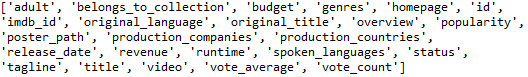
\includegraphics[width=\textwidth]{images/Raw_dataset_headers.png}
	\caption{Columns of the file \textit{movies-metadata.csv}}
\end{figure}

%Due to the multitude of attributes, it is essential to extract the relevant values for the implementation of a well-functioning classifier. Many values have no effect on the financial success of a movie and can therefore be ignored. This includes, for example, the columns...

The structure of the data attributes varies. String, Float values, List of JSON objects. All of those values need special treatment in preprocessing. More later on.


\section{Basic data exploration}
Taking a deeper look at the data. Quality varies vary much. String values oftentimes missing, encoded wrong. Especially for older movies a lot of data is missing. For numerical values no info about currency. Complicated because later computations will rely heavily on revenue and budget data. Diving deeper into those can see a lot of values are missing or containing zero (get the number from pandas). Must be taken into account for preprocessing. Average budget value, average revenue (without zero). Correlation between revenue and budget. The most common genre is... . Average number of actors per movie.

Back to revenue and budget take into account that this is data from past 60 years. A lot of things changed in movie economics (prices, consumer Verhalten, globalization). Introduced new column, productivity value
A lot of values are scaled wrongly. Little example with 2 movies. 2000000 in revenue is just stated as 2, don't know the scale of data. Will be a big problem

\begin{itemize}
	\item In slides named: "structure and size of data"
	\item min. 1 Page
	\item Selection: 
	\begin{itemize}
		\item What data is available?
		\item What do I know about the provenance of the data?
		\item What do I know about the quality of the data?
		\item Wrong values, lot of null values
	\end{itemize}
	\item Exploration
	\begin{itemize}
		\item Get an initial understanding of the data
		\item Calculate basic summarization statistics
		\item Visualize the data
		\item Identify data problems such as outliers, missing values, duplicate records
		\item problem with number scales, data formats, truth of contents
	\end{itemize}
\end{itemize}

Main issue quality of data. Further explained in preprocessing...
